\section{Overview of the Project InsightCAE}

\subsection{Concept and Parts of the Project}

The InsightCAE builds on top of available open-source engineering analysis tools (though closed-source tools could be used as well). The most used tool by far is the CFD software OpenFOAM.

For certain tasks, custom extensions to these tools are required. InsightCAE contains a selection of extensions, which are included in the distribution packages, when these are created.

The core of the project is the toolkit library. It contains the implementation of core classes in workflow management as the parameter set storage and tools and result set storage classes and handling tools.
The toolkit library also maintains a list of available analysis modules, which is dynamically extensible by loadable add-ons.

Finally, on top of the toolkit library, custom analysis modules can be created.
The InsightCAE base distribution contains a number of generic analysis modules as the "Numerical Wind Tunnel" module and some generic test case analyses like flat plate, channel flow, pipe flow and so on. These might serve as examples for custom implementations.


\begin{figure}[h!]
\centering
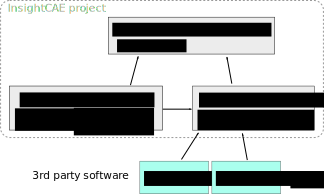
\includegraphics[width=0.75\linewidth,keepaspectratio]{\currfileabsdir/figs/intro/insightcae-structure}
\caption{Structure of the InsightCAE project}
\label{fig:insightcae-structure}
\end{figure}


\subsection{Terms and Defintions}

\paragraph{Simulation App, Analysis}

InsightCAE bundles tools to create automated simulation procedures. These procedures can be written in Python or C++. The term \textbf{analysis}, \textbf{workflow module} or \textbf{Simulation App} is used for such a procedure.

Actually, an analysis is like a function in programming: it gets input parameters, executed some actions (e.g. a numeric simulation) and returns a results data structure.

InsightCAE provides a GUI to edit the parameter sets and also tools to work with the result sets. E.g. convert the result set into a PDF report.

\paragraph{Parameter Set}

The analysis modules need input data, i.e. parameters. All parameters for a module are grouped together in a parameter set. Parameter sets are stored in XML files in human readable format (extension *.ist). They can also be edited in a GUI editor (application workbench).

Many analysis modules need external files (like CAD data in STL or any other format). These files can simply be referred in a parameter set by their relative path (relative to the *.ist-file containing the reference) or absolute path. It is also possible to embed the external files into the XML file in an base64-encoded form. This simplifies transfer of analysis setup from one computer to another, e.g. for remote execution.

\paragraph{Result Set}

The result of an analysis is returned in a \textbf{result set}. This is a hierarchical data structure which contains nodes like scalar values, charts, contour plots, images, tables or similar entities.
It can be stored on disk in XML format.
There is also a renderer which converts a result set into a PDF report.

\paragraph{Case Element}

The setup of CFD-runs is put together from a number of so-called \textbf{case elements}. Each case element represents some functional feature. It might be a boundary condition or a turbulence model or something similar. A case element is not necessarily associated with a certain configuration file but can modify multiple configuration files of a CFD case configuration.

There is also an editor for composing OpenFOAM cases from the available case elements: the OpenFOAM Case Builder.


\begin{itemize}
\item Solver extensions
\item OpenFOAM Case Builder
\item Workbench
\end{itemize}


